\documentclass[10pt]{article}
\usepackage[usenames]{color} %used for font color
\usepackage{amssymb} %maths
\usepackage{amsmath} %maths
\usepackage[ruled,linesnumbered]{algorithm2e}
\usepackage[utf8]{inputenc} %useful to type directly diacritic characters

\usepackage{graphics}
\usepackage{adjustbox}
\usepackage{float}
%\usepackage{listings}


\usepackage[usenames]{color} %used for font color
\usepackage{amssymb} %maths
\usepackage{amsmath} %maths
\usepackage[ruled,linesnumbered]{algorithm2e}
\usepackage[utf8]{inputenc} %useful to type directly diacritic characters
\usepackage{listings}
\usepackage{graphics}
\usepackage{adjustbox}
\usepackage{float}

% Default fixed font does not support bold face
\DeclareFixedFont{\ttb}{T1}{txtt}{bx}{n}{12} % for bold
\DeclareFixedFont{\ttm}{T1}{txtt}{m}{n}{12}  % for normal

% Custom colors
\usepackage{color}
\definecolor{deepblue}{rgb}{0,0,0.5}
\definecolor{deepred}{rgb}{0.6,0,0}
\definecolor{deepgreen}{rgb}{0,0.5,0}

\usepackage{listings}

% Python style for highlighting
\newcommand\pythonstyle{\lstset{
		language=Python,
		basicstyle=\ttm,
		otherkeywords={self},             % Add keywords here
		keywordstyle=\small\ttb\color{deepblue},
		emph={MyClass,__init__},          % Custom highlighting
		emphstyle=\ttb\color{deepred},    % Custom highlighting style
		stringstyle=\small\color{deepgreen},
		frame=tb,                         % Any extra options here
		showstringspaces=false            % 
}}


% Python environment
\lstnewenvironment{python}[1][]
{
	\pythonstyle
	\lstset{#1}
}
{}

% Python for external files
\newcommand\pythonexternal[2][]{{
		\pythonstyle
		\lstinputlisting[#1]{#2}}}

% Python for inline
\newcommand\pythoninline[1]{{\pythonstyle\lstinline!#1!}}



\begin{document}
	\begin{raggedright}	
		Michael Lan \\
		Lingfei Zeng \\
		Xunjie Zhu \\
	\end{raggedright}


	
Stage3 - The Implementation Stage. \\

\begin{itemize}
	\item Novelty
\end{itemize}
Users can already find tweets related to their topic by searching for keywords or hashtags related to their topic. However, this project will allow users to find tweets that are both semantically and structurally similar to their tweets, not just related to the topic of those tweets. Users will also be recommended hashtags, such as those of ‘intermediate popularity’, which users do not include in their tweets, but which are topically related to their tweets.

\begin{itemize}
	\item Usefulness
\end{itemize}
This project will allow users to find which tweets and hashtags are similar to their own tweets. Thus, this project aims to bridge different Twitter communities by finding ‘hidden’ connections between them based on different measures of similarity. This will facillitate communication between previously isolated communities.
\begin{itemize}
	\item Development Environment
\end{itemize}	
This project is developed with Python language and the Linux operating system. \\
%Building the corresponding relational tables, according to the proposed ER model described in the previous phase %enforcing the different integrity constraints.  
The deliverables for this stage include the following items:\\\\
Section 1. Evaluation of tweet dissimilarity by Extended Edit Distance integrated Word2Vec (EDW), and clustering by the distance value (Implemented and written by Lingfei Zeng)
\begin{itemize} 
\item{}
Sample small data snippet. \\
The input data are plain text of tweet contents. The plain text can be converted by Json file scraped from the webpage. In this section, the sample data are the scraped tweets in csv file, downloaded from http://followthehashtag.com/datasets/, named "USA Geolocated tweets". It contains 20,000 tweets and here is the sample of the data are in Table~\ref{Table1}:


   
\item{}
Sample small output\\
In the distance evaluation job, the output of the system is distance value of two tweets, ranging from 0 to 1 . After clustering by  k-medoids or hierarchical clustering method, the output are the clusters of tweets. 
   
\item{}
Working code

\begin{python}
# Disimilarity evaluation algorithm Extended Edit 
# Distance integrated Word2Vec (EDW)

def sentence_to_word(sentence):
    sentence = re.sub("[^a-zA-Z]", " ", sentence.lower())
    words = WORD.findall(sentence)
    return words

def edit_distance(s1, s2):
    words_1 = sentence_to_word(s1)
    words_2 = sentence_to_word(s2)

    m=len(words_1)+1
    n=len(words_2)+1

    tbl = {} 
    bestMove={}
    for i in range(m):
	    tbl[i,0]=i
	    bestMove[i, 0] = 'D'

    for j in range(n):
        tbl[0,j]=j
        bestMove[0, j] = 'I'

    for i in range(1, m):
        for j in range(1, n):
            if words_1[i-1] == words_2[j-1]:
            cost = 0
            minVal = 10000000
                if tbl[i, j - 1] + 1 < minVal:
                    minVal = tbl[i, j - 1] + 1
                    bestMove[i, j] = 'D'
                if tbl[i - 1, j] + 1 < minVal:
                    minVal = tbl[i - 1, j] + 1
                    bestMove[i, j] = 'I'
                if tbl[i - 1, j - 1] + cost < minVal:
                    minVal = tbl[i - 1, j - 1] + cost
                    bestMove[i, j] = ' ' 

            else:
                try:
                    word2vec_cost = 1 - model.similarity(
                    words_1[i - 1],
                     words_2[j - 1])
                except KeyError, e:
                    word2vec_cost = 1  

                cost = 2*word2vec_cost

                minVal = 10000000
                if tbl[i, j - 1] + 1 < minVal:
                    minVal = tbl[i, j - 1] + 1
                    bestMove[i, j] = 'D'
                if tbl[i - 1, j] + 1 < minVal:
                    minVal = tbl[i - 1, j] + 1
                    bestMove[i, j] = 'I'
                if tbl[i - 1, j - 1] + cost < minVal:
                    minVal = tbl[i - 1, j - 1] + cost
                    bestMove[i, j] = 'R'

                tbl[i, j] = minVal

    iTmp = i
    jTmp = j
    counting = 0
    while True:
        if bestMove[iTmp, jTmp] == 'R' or bestMove[iTmp, jTmp] == ' ':
            if bestMove[iTmp, jTmp] == 'R':
            counting += 1
            iTmp -= 1
           jTmp -= 1
        elif bestMove[iTmp, jTmp] == 'D':
            jTmp -= 1
        elif bestMove[iTmp, jTmp] == 'I':
            iTmp -= 1
        if iTmp == 0 or jTmp == 0:
            break

    counting += max(m-1,n-1)
    return tbl[i,j]/counting

\end{python}


\item{}
Demo and sample findings\\
The performance of EDW algorithm is evaluated by published paired-wised benchmark data set \cite{O'shea:2014:NBD:2560566.2537046}  first. Several benchmarking paired sentences with different similarities were tested with our algorithm. The results together with the comparison of the similarities reported in the literature are shown in Table~\ref{Table2}. Since the benchmarking uses different scale of core system, the table lists the levels of similarities of each sentence pairs directly. Besides are the distance score generated by EDW, ranging from 0-1, from least similar to identical. From the comparison we can see that the EDW calculated the distance between benchmarking sentences in high accuracy. \\\\

\begin{table}[]
	\centering
	\caption{Data Snippet}
	\label{Table1}
	\begin{tabular}{llllll}
		\cline{1-2}
		\multicolumn{1}{|l|}{Index} & \multicolumn{1}{l|}{Tweet contents}                                                                                                                                                               &  &  &  &  \\ \cline{1-2}
		\multicolumn{1}{|l|}{1}     & \multicolumn{1}{l|}{I'm at,@DunkinDonuts in Lithonia, GA https://t.co/d6IU15ig5J}                                                                                                                 &  &  &  &  \\ \cline{1-2}
		\multicolumn{1}{|l|}{2}     & \multicolumn{1}{l|}{Cleared:,Closure on \#US1 SB at South of Olden Ave}                                                                                                                           &  &  &  &  \\ \cline{1-2}
		\multicolumn{1}{|l|}{3}     & \multicolumn{1}{l|}{\begin{tabular}[c]{@{}l@{}}Want to,work in \#Burlington, MA? View our latest opening: \\ https://t.co/qwwWQt0DMj,\#Healthcare \#Job \#Jobs \#Hiring \#CareerArc\end{tabular}} &  &  &  &  \\ \cline{1-2}
		&                                                                                                                                                                                                    
	\end{tabular}
\end{table}



\begin{table}[]
	\centering
	\caption{Distance score generated by EDW, compared with reported benchmarking}
	\label{Table2}
	\begin{tabular}{|l|l|l|ll}
		\cline{1-3}
		Sentence pair                                                                                                                                                                                     & \begin{tabular}[c]{@{}l@{}}Semantic similarities\\ reported by [1]\end{tabular} & \begin{tabular}[c]{@{}l@{}}Distance sore\\ by EDW\end{tabular} &  &  \\ \cline{1-3}
		\begin{tabular}[c]{@{}l@{}}Midday is 12 o'clock in the middle of the day.\\ Noon is 12 o'clock in the middle of the day.\end{tabular}                                                             & Identical                                                                   & 0.081319882                                                 &  &  \\ \cline{1-3}
		\begin{tabular}[c]{@{}l@{}}A boy is a child who will grow up to be a man.\\ A lad is a young man or boy.\end{tabular}                                                                             & Related                                                                     & 0.59221011                                                  &  &  \\ \cline{1-3}
		\begin{tabular}[c]{@{}l@{}}A hill is an area of land that is higher than the land\\ that surrounds it.\\ A mound of something is a large rounded pile of it.\end{tabular}                         & Vaguely similar                                                             & 0.76921332                                                  &  &  \\ \cline{1-3}
		\begin{tabular}[c]{@{}l@{}}Cord is strong, thick string.\\ A smile is the expression that you have on your \\ face when you are pleased or amused, or when you\\ are being friendly.\end{tabular} & Unrelated                                                                   & 0.91587261                                                  &  &  \\ \cline{1-3}
	\end{tabular}
\end{table}      

Then using the tweet data set, a pair-wised distance matrix was generated based on the score calculated by EWD. This distance matrix was utilized to do the clustering with k-medoids or hierarchical clustering method. The functions are available in related Python packages Kmedoids and Scipy. For k-medoids method, the outputs are  index of tweets in different clusters. For hierarchical clustering method, the outputs are tweet clusters and a dendrogram. A sample output by the k-medoids method were shown in the Table~\ref{Table3}. The tweets have been grouped into 3 clusters and the similarities of tweets in the same clusters are very high. A sample output of dendrogram of 100 tweets generated by hierarchical clustering are shown in Figure \ref{fig1}. 
     

\begin{table}[]
	\centering
	\caption{Sample result of tweet clusters }
	\label{Table3}
	\begin{tabular}{|l|l|lll}
		\cline{1-2}
		Tweet contents                                                                                                                                                                & \begin{tabular}[c]{@{}l@{}}Cluster \\ label\end{tabular} &  &  &  \\ \cline{1-2}
		I'm at,@DunkinDonuts in Lithonia, GA https://t.co/d6IU15ig5J                                                                                                                  & 0                                                        &  &  &  \\ \cline{1-2}
		I'm at,@InNOutBurger in Long Beach, CA https://t.co/uqmEomzVKZ                                                                                                                & 0                                                        &  &  &  \\ \cline{1-2}
		I'm at Home,https://t.co/fDCP5atErT                                                                                                                                           & 0                                                        &  &  &  \\ \cline{1-2}
		\begin{tabular}[c]{@{}l@{}}I'm at Los Angeles,International Airport (LAX) - @flylaxairport in\\  Los Angeles, CA,https://t.co/rCVIJrXCMX\end{tabular}                         & 0                                                        &  &  &  \\ \cline{1-2}
		I'm at Twerk in,Horsham, PA https://t.co/VRmWIJssIC                                                                                                                           & 0                                                        &  &  &  \\ \cline{1-2}
		Cleared:,Closure on \#US1 SB at South of Olden Ave                                                                                                                            & 1                                                        &  &  &  \\ \cline{1-2}
		\begin{tabular}[c]{@{}l@{}}Cleared:,Incident on \#I87NYSThruway NB at Exit 21 (I-87)\\  - Catskill (Rte 23)\end{tabular}                                                      & 1                                                        &  &  &  \\ \cline{1-2}
		\begin{tabular}[c]{@{}l@{}}Want to,work in ? View our latest opening: https://t.co/47mSniYiPU \\ \#Hospitality,\#Veterans \#Job \#Jobs \#Hiring \#CareerArc\end{tabular}      & 2                                                        &  &  &  \\ \cline{1-2}
		\begin{tabular}[c]{@{}l@{}}Want to,work in \#Burlington, MA? View our latest opening: \\ https://t.co/qwwWQt0DMj,\#Healthcare \#Job \#Jobs \#Hiring \#CareerArc\end{tabular}  & 2                                                        &  &  &  \\ \cline{1-2}
		\begin{tabular}[c]{@{}l@{}}Want to,work in \#Charlotte, NC? View our latest opening: \\ https://t.co/nkrJjulisQ,\#BusinessMgmt \#insurance \#Job \#Jobs \#Hiring\end{tabular} & 2                                                        &  &  &  \\ \cline{1-2}
		\begin{tabular}[c]{@{}l@{}}Want to,work in \#FALLSCHURCH, VA? View our latest opening: \\ https://t.co/sgxNmVAkQl,\#Healthcare \#Job \#Jobs \#Hiring \#CareerArc\end{tabular} & 2                                                        &  &  &  \\ \cline{1-2}
	\end{tabular}
\end{table}


\begin{figure}[h]
	\caption{Dendrogram generated by EDW and hierarchical clustering)}
	\centering
	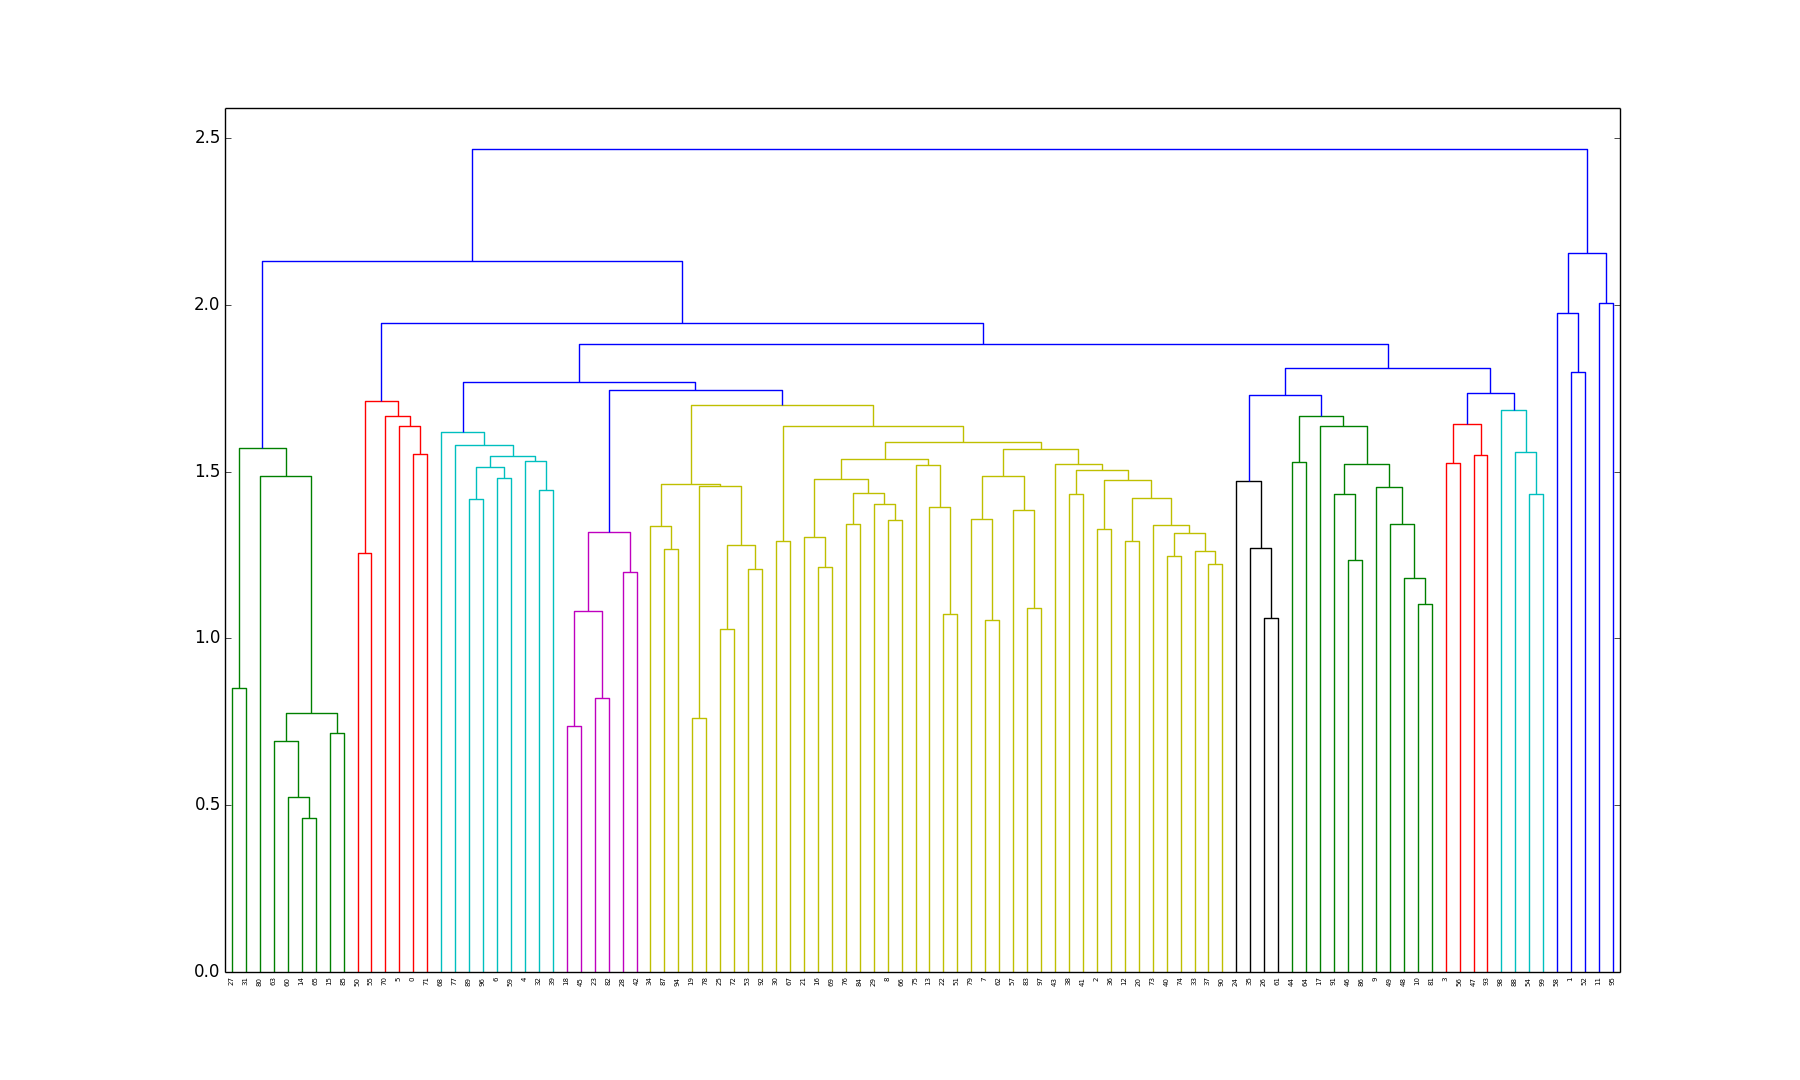
\includegraphics[scale=0.3]{figure_1_hcluster.png}
	\label{fig1}
\end{figure}


\end{itemize}
{\bf Section 2. Evaluation of tweet similarity by TF-IDF based document2vec and Hierarchical Clustering (Implemented by Xunjie Zhu and written by Michael Lan) }

\begin{itemize}
	\item Sample Small Data Snippet (This is a subset 3 tweets out of thousands of tweets used)
\end{itemize}
211 : RT @KCONTV: Fans dancing in front of the @HondaCenter before the \#BTSinAnaheim concert! \#TWTinAnaheim \#BTS https://t.co/QAVEt0uqYn
212 : RT @BTS\_V\_sana:   02line(01)ARMY  all    \#ARMY  \#BTSRT  \#RT https://
213 : RT @bangtanitl: \#BTS was mentioned on Kangnam Style, 170331 https://t.co/uL8yrSGBJB https://t.co/qJ0IINaTrH

\begin{itemize}
	\item Sample Small Data Output
\end{itemize}
The word and paragraph vectors, along with the document-term frequency matrix, are huge, so we did not include them in Phase 3 write-up. Additionally, they are only intermediate outputs. The dendrogram of the clustering results is the final output, and a visual and description of it is given below the pipeline description in this section.

\begin{itemize}
	\item Pipeline Description
\end{itemize}
Since it would be quite lengthy to include all the code used, only the hierarchical clustering algorithm code has been given at the end of this section. Also, the bipartite graph and Simrank code was completed but are not part of the main pipeline yet, so only a histogram of their output is given; the code is not included. The rest of the code can be given upon request, and may be included in the final report. The pipeline is briefly described:
\\\\
The data crawler uses a listener to find new tweets that contain certain keywords or hashtags, collectively called a ‘filter’. To find tweets that are related to certain topics but do not necessarily contain the hashtags of those topics, we first gathered tweets containing initial keywords. New keywords, hashtags, and topics were found from in this first iteration of tweets, and were added to the filter. Then, we ran the data crawler again using this new filter, and repeated this multiple times. Essentially, we used previous iterations of keywords or hashtags to find new topics, and we only ran clustering on the tweets found in the final iteration. Each iteration is called a ‘generation’.
\\\\
There were two separate methods we used to find new topics: 
1)We took the 10 most frequent new, non-trivial keywords hashtags found in this first iteration of tweets and added them to the filter 
2) We used LDA to find new topics. 
IE)
Filter in Gen 1: music, concerts
Filter in Gen 2: music, concerts, classical, metal
Filter in Gen 3: music, concerts, classical, metal, bach
\\\\
Later, the crawler and topic finding scripts will be deployed to a linux server to be run periodically. This will be implemented by crontab.
\\\\
The pipeline is described as follows:
\begin{enumerate}
	\item Start up a listener of incoming tweets. Uses the Tweepy library to connect to Twitter Streaming API. Outputs a JSON text file of data
	\item Read a JSON text file and outputs a file of tweets
	\item Use term frequency and latent dirichlet allocation respectively to find new topics from existing tweets
	\item Read file of tweets and uses regular expressions to do some preprocessing
	\item  Train word vector and tf-idf weighted sum of word vector to form document vector. Computes similarity between tweets. Outputs word and paragraph vectors
	\item Cluster the tweets into topics and outputs a dendrogram
\end{enumerate}

\begin{itemize}
	\item Interesting findings in Dendrogram
\end{itemize}
Since there were thousands of tweets that were gathered, we created a dendrogram for 100 tweets. There appear to be two main groups, and within the red group, there were 4 main subgroups. This sample shows that our algorithms work. However, since we did not input in meaningful data yet, and since this dendrogram only shows 100 of thousands of tweets, we do not expect this sample to give meaningful results. Later, we will gather better data and perform an analysis.

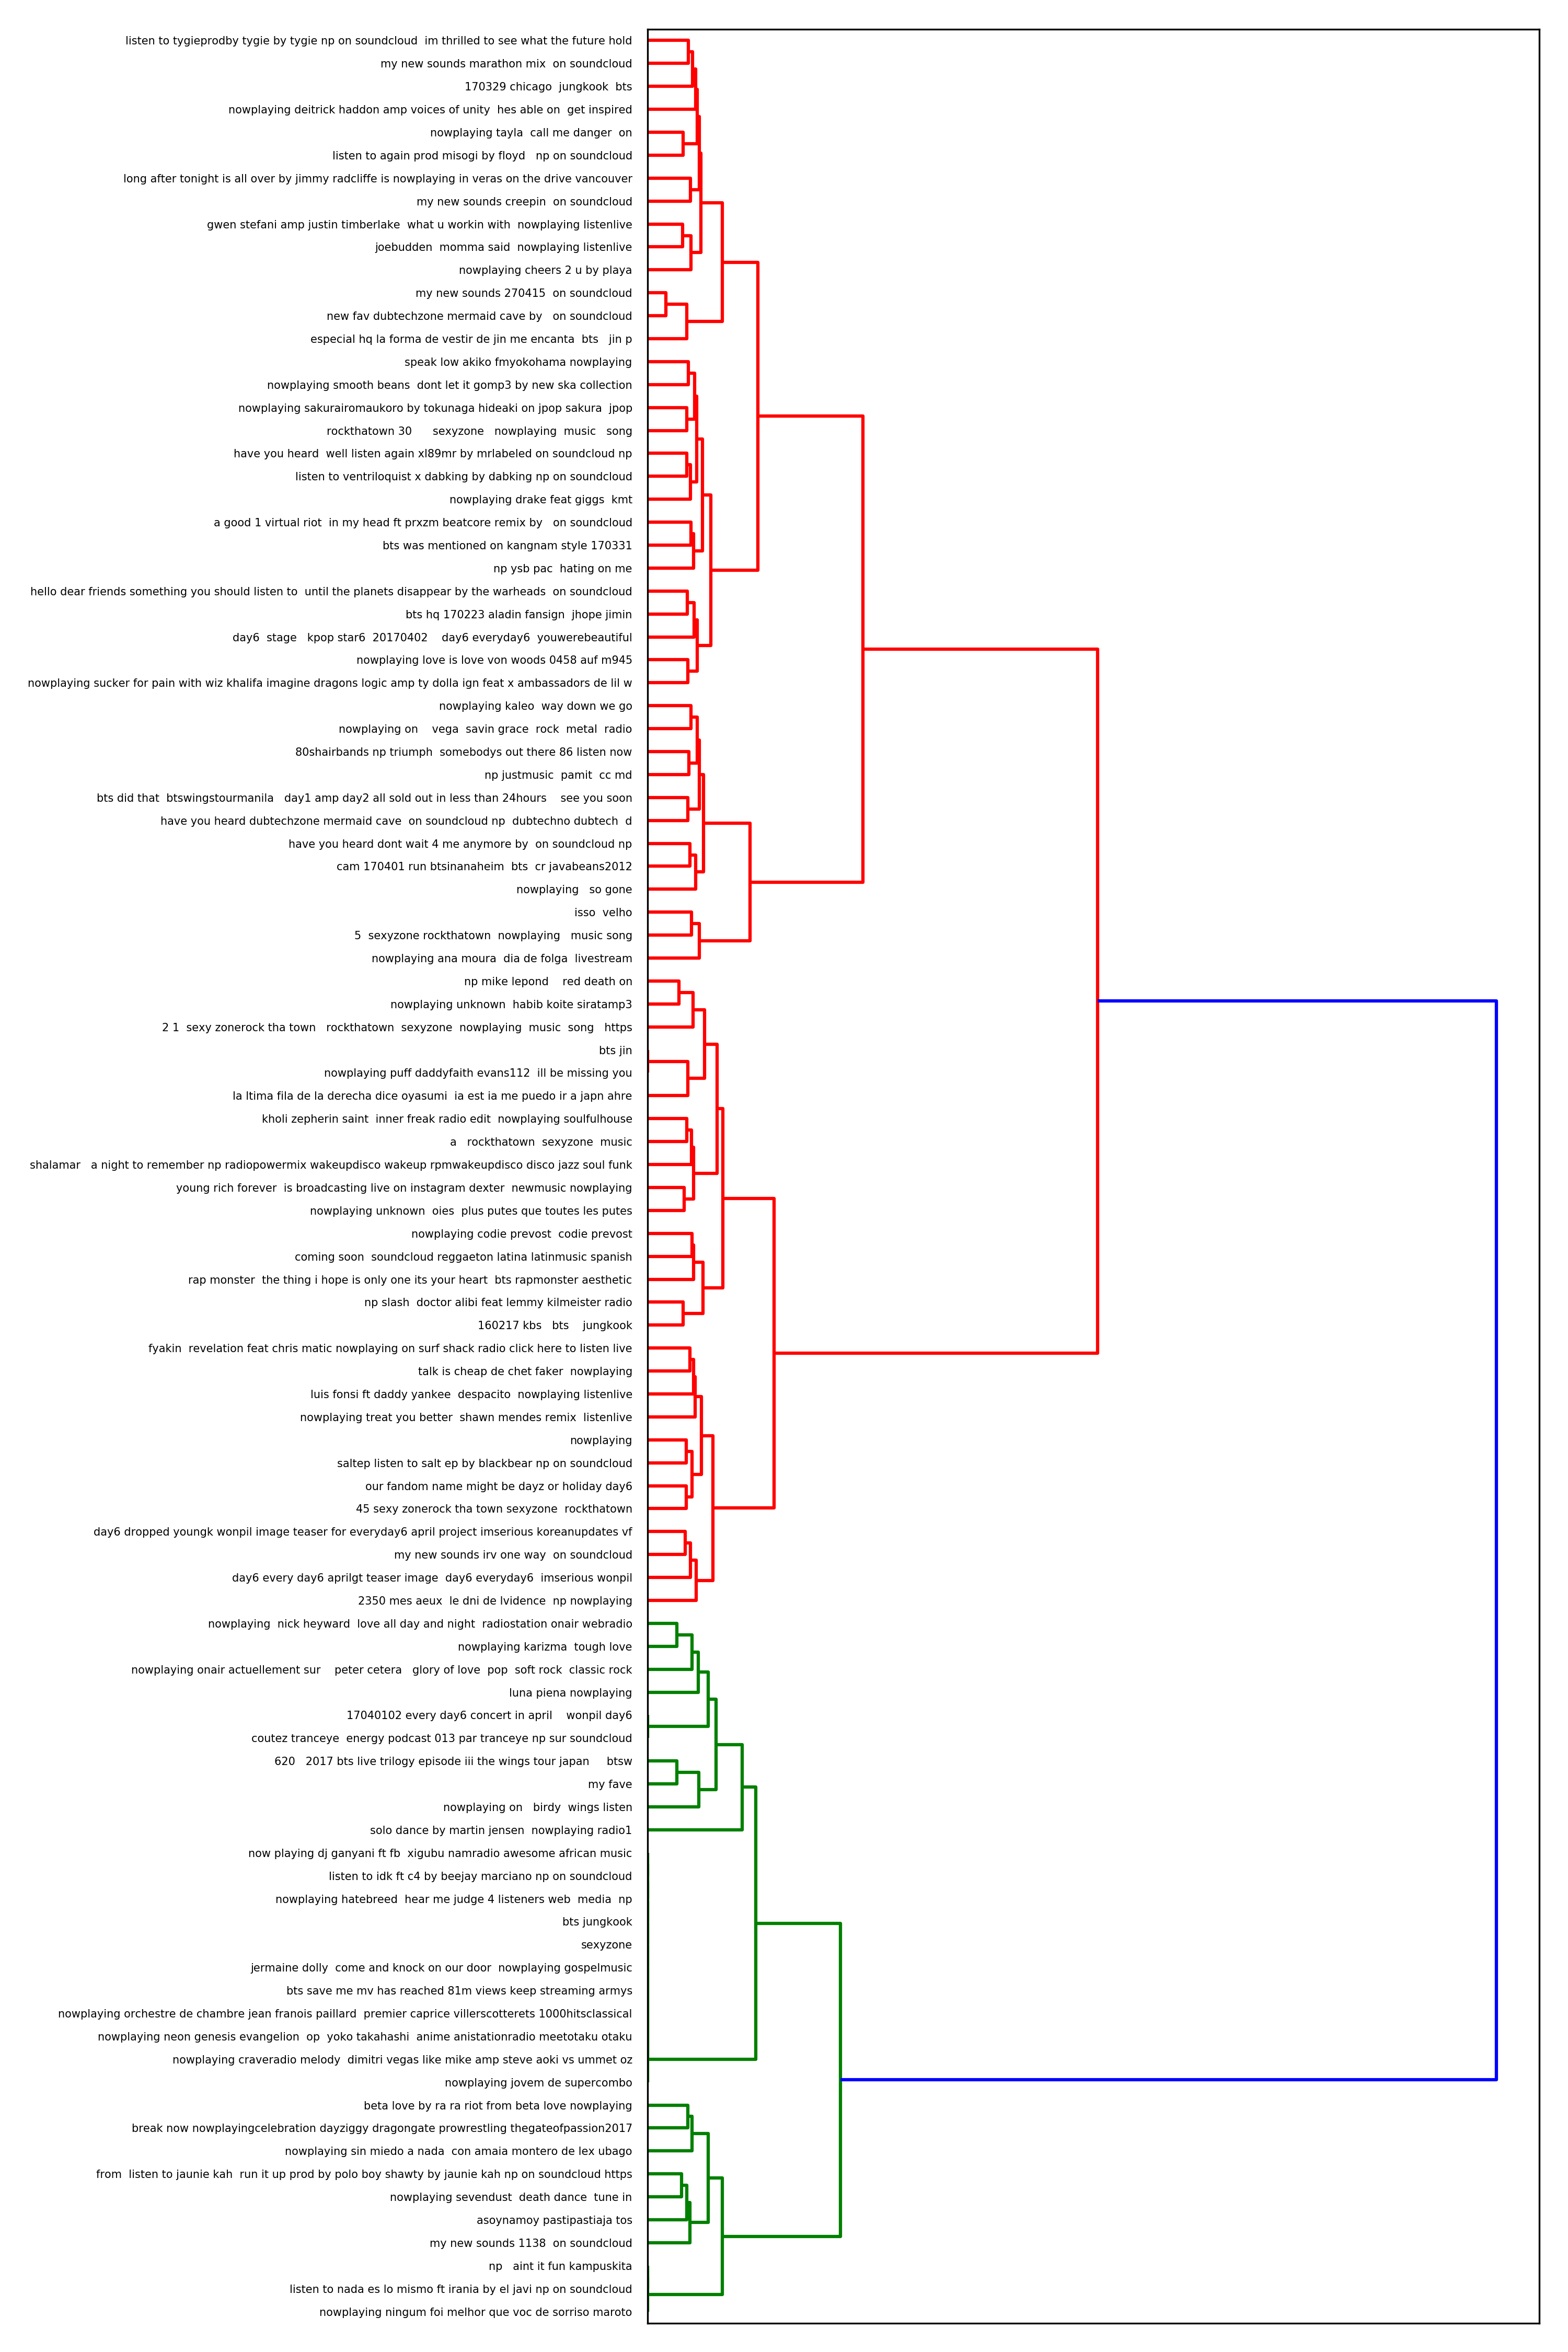
\includegraphics[scale=0.5]{clusters.png}

\begin{itemize}
	\item Working Code
\end{itemize}

\begin{python}
class HierarchicalClusterer(object):
    def __init__(
            self,
            distance_matrix,
            linkage_function,
            minium_clusters=2):
        self.distance_matrix = distance_matrix
        self.linkage_function = linkage_function
        self.minium_clusters = minium_clusters

    def build_clusters(self):
        print 'a'

    def do_link_clustering(self, cluster_id_list, cluster_nodes):

        def small_big(first, second):
             if first < second else (second, first)

        def merge(cluster1,
                  cluster2,
                  distance,
                  cluster_ids,
                  cluster_nodes):
            cluster1, cluster2 = small_big(cluster1, cluster2)
            cluster_ids[cluster1].extend(cluster_ids[cluster2])
            cluster_ids[cluster2] = []
            node = Node()

            if cluster_nodes[cluster1]:
                node.left = cluster_nodes[cluster1]
                cluster_nodes[cluster1].parent = node
            else:
                node.left_instance = cluster1

            if cluster_nodes[cluster2]:
                node.right = cluster_nodes[cluster2]
                cluster_nodes[cluster2].parent = node
            else:
                node.right_instance = cluster2

            node.set_height(distance, distance)
            cluster_nodes[cluster1] = node

        length = self.distance_matrix.shape[0]
        cluster_number = self.distance_matrix.shape[0]
        distance_list = [
            ClusterPair(first,
            second,
            self.distance_matrix[first][second], 1, 1)
            for first in range(length) for second in range(first + 1, 
            length)]

        distance_queue = MyHeap(
            initial=distance_list,
            key=lambda x: x.distance)

        while cluster_number - self.minium_clusters > 0:
            pair = distance_queue.pop()
            if not pair:
                break

            if not valid_pair(pair, cluster_id_list):
                continue

            merge(pair.cluster1, pair.cluster2,
             pair.distance, cluster_id_list, cluster_nodes)

            for index in range(length):
                if index != pair.cluster1 \
                        and cluster_id_list[index]:
            cluster1, cluster2 = \
                small_big(cluster1, cluster2)

                    new_distance = self.linkage_function(
                        self.distance_matrix,
                        cluster_id_list[smaller],
                        cluster_id_list[bigger])

                    distance_queue.push(ClusterPair(
                        smaller,
                        bigger,
                        new_distance,
                        len(cluster_id_list[smaller]),
                        len(cluster_id_list[bigger])))

            cluster_number -= 1

\end{python}

{\bf Section 3. Evaluation by SimRank (Implemented by Michael Lan) }
This was written in Python 2.7, using the Sublime Text Editor. We gathered data, called ‘Dataset 8’, which belongs to 2 very different communities: Music and Politics. This dataset uses the initial filter: 
$$\#music, \#concert, \#politics, \#trump, \#russia, \#brexit$$

The Gaming hashtags \#gaming, \#gamers, \#pc, and \#xbox were also included, but they did not yield many tweets.
\\\\
Sample Findings: We tested to see if the system would say that tweets or hashtags about music would be similar to music-related tweets and hashtags, and did the same with politics. The Demo Video in Phase 4 shows that the system was able to do this.
\\\\
Since the rest of the code has many lines, it is not included in this report. The small data snippet (around 37 Mb), small sample output and the code are uploaded on Github: 
https://github.com/circlefive05/SimRank-on-Twitter-UI
\\\\
Some more information can be found on the file ‘More on SimRank.doc’ on [...]
\\\\
Implementation Steps:
\begin{enumerate}
	\item Using the Tweepy API, start up a listener of incoming tweets. Two iterations: first iteration uses a set of ‘initial hashtags’. Second iteration uses the top 25\% most frequent hashtags from the previous iteration’s tweets, plus the hashtags from the previous iteration’s filter, to filter tweets in the second iteration. A JSON file is outputted, and tweets, in plain text, are extracted from this using the Pandas library.
\item Create bipartite graph G. Use positive ID integers for tweets, and negative ID integers for hashtags. Create an adjacency matrix M such that each node is assigned an index id.
\item Compute $M^k$ for even numbers up to k = Kmax. Assuming sparsity, choose Kmax = 4. Sum up these $M^k$. Take the nonzero entries, the chosen pairs, of the sum. Run SimRank on the chosen pairs. Use pickle to store the graph, the ID-to-node hash tables, and the scores hash table. 
\end{enumerate}	
The iterative gathering approach obtains tweets which are structurally similar to the filter, but does not restrict the data to only finding tweets that contain hashtags in the filter. This is better than blindly gathering Listener. We only demonstrate a sample with a small amount of data, so the results are not as strong. Also, since the data consists of new tweets, the results depends on what’s trending at the time of collection.

%\bibliographystyle{abbrv}
%\bibliography{stage3}  % sigproc.bib is the name of the Bibliography in this case
\end{document}